\section{Observer-induced irreversibility of filtered signals}\label{sec:theory}

\subsection{Setting and the time-reversal decomposition}\label{sec:decomp}

Any linear filter of a stationary multichannel signal produces a lag-one antisymmetry that splits exactly into an observer term and a physical term. Let $u_t=(u^1_t,\dots,u^P_t)$ be a jointly stationary input with cross-covariances
\begin{equation}
\gamma_{pq}(\tau)=\mathrm{Cov}(u^p_{t+\tau},u^q_t),\qquad \gamma_{qp}(\tau)=\gamma_{pq}(-\tau),
\end{equation}
and let an observer form the state $y(t)=(y_1,\dots,y_m)$ from causal filters,
\begin{equation}
y_i(t)=\sum_{a\ge0}k_i(a)\,u^{p_i}_{t-a},
\end{equation}
where $p_i$ labels the input channel of observable $i$; a trailing mean of width $w_i$ has $k_i(a)=1/w_i$ for $0\le a<w_i$. With $C(s)=\mathrm{Cov}[y(t+s),y(t)]$, time reversibility of a stationary process requires $C(s)=C(s)^\top$ for all $s$; for a Gaussian process the condition is also sufficient, because second moments fix its law, and reversibility criteria for linear non-Gaussian processes are classical \cite{weiss1975,tong2005,chan2006}. The leading time-reversal-odd statistic is the standardized lag-one antisymmetry
\begin{equation}
\omega_{ij}=\frac{C_{ij}(1)-C_{ji}(1)}{2\sqrt{C_{ii}(0)C_{jj}(0)}} .\label{eq:omega}
\end{equation}
In standardized coordinates $\omega_{ij}$ is minus the mean signed area swept per step by the trajectory in the $(y_i,y_j)$ plane, i.e.\ the discrete-time area-enclosing rate \cite{ghanta2017,gonzalez2019}, closely related to the cycling frequencies of probability-flux analysis \cite{gradziuk2019,battle2016}; for the linear Markov model fitted to $y$ it sets the stationary current (Sec.~\ref{sec:factor}). Define the cross-correlation of two kernels,
\begin{equation}
K_{ij}(m)=\sum_a k_i(a)\,k_j(a+m),\qquad K_{ji}(m)=K_{ij}(-m),
\end{equation}
and write $f^\pm$ for the even and odd parts of a sequence, $f^\pm(m)=\tfrac12[f(m)\pm f(-m)]$. For a covariance sequence $\gamma$ we write $\Delta\gamma^\pm\equiv\Delta(\gamma^\pm)$ for the difference operator applied to its even and odd parts, $(\Delta\gamma^\pm)(m)=\gamma^\pm(m+1)-\gamma^\pm(m-1)$; $\Delta\gamma^+$ is odd and $\Delta\gamma^-$ is even.

\begin{proposition}[Time-reversal decomposition]\label{prop:decomp}
With $\gamma\equiv\gamma_{p_ip_j}$ and $\Delta\gamma(m)=\gamma(m+1)-\gamma(m-1)$,
\begin{equation}
C_{ij}(1)-C_{ji}(1)=\sum_m K_{ij}(m)\,\Delta\gamma(m).\label{eq:decomp}
\end{equation}
Consequently $\omega_{ij}=O_{ij}+P_{ij}$ with
\begin{align}
O_{ij}&=\frac{1}{2\sigma_i\sigma_j}\sum_m K^-_{ij}(m)\,\Delta\gamma^+(m),\label{eq:O}\\
P_{ij}&=\frac{1}{2\sigma_i\sigma_j}\sum_m K^+_{ij}(m)\,\Delta\gamma^-(m),\label{eq:P}
\end{align}
$\sigma_i^2=C_{ii}(0)$. Under time reversal of the input, $O_{ij}\to O_{ij}$ and $P_{ij}\to-P_{ij}$.
\end{proposition}

\begin{proof}
Substituting $b=a+m$ in $C_{ij}(s)=\sum_{a,b}k_i(a)k_j(b)\,\gamma(s-a+b)$ gives $C_{ij}(s)=\sum_mK_{ij}(m)\gamma(s+m)$. With $K_{ji}(m)=K_{ij}(-m)$ and $\gamma_{p_jp_i}(\tau)=\gamma(-\tau)$, $C_{ji}(1)=\sum_mK_{ij}(m)\gamma(m-1)$, which is Eq.~\eqref{eq:decomp}. Write $K_{ij}=K^+_{ij}+K^-_{ij}$ and $\Delta\gamma=\Delta\gamma^++\Delta\gamma^-$. The difference operator maps even sequences to odd ones and odd sequences to even ones, so the products $K^+_{ij}\Delta\gamma^+$ and $K^-_{ij}\Delta\gamma^-$ are odd in $m$ and sum to zero. The surviving products, $K^-_{ij}\Delta\gamma^+$ (odd times odd) and $K^+_{ij}\Delta\gamma^-$ (even times even), are even and give Eqs.~\eqref{eq:O} and \eqref{eq:P}. Time reversal maps $\gamma_{pq}(\tau)\to\gamma_{pq}(-\tau)$, hence $\gamma^+\to\gamma^+$ and $\gamma^-\to-\gamma^-$, and leaves $\sigma_i^2=\sum_mK_{ii}(m)\gamma^+_{p_ip_i}(m)$ unchanged.
\end{proof}

The observer term needs kernels whose cross-correlation is not symmetric, i.e.\ windows with different temporal centers; it is built from the time-symmetric part of the input covariances. The physical term needs an odd cross-covariance between input channels, i.e.\ genuine time asymmetry of the input. Proposition~\ref{prop:decomp} yields a model-free estimator: rebuilding the features from the time-reversed input gives $\omega^{\rm rev}_{ij}=O_{ij}-P_{ij}$, so
\begin{equation}
O_{ij}=\tfrac12(\omega_{ij}+\omega^{\rm rev}_{ij}),\qquad P_{ij}=\tfrac12(\omega_{ij}-\omega^{\rm rev}_{ij}).\label{eq:estimator}
\end{equation}
For nonlinear features (logarithms, running maxima) the decomposition holds to linear order. Equation~\eqref{eq:estimator} nevertheless remains an exact split of any statistic into its time-reversal-even and time-reversal-odd parts, and Sec.~\ref{sec:market} measures how close this split is to the linear one.

\begin{figure*}[t]
\centering
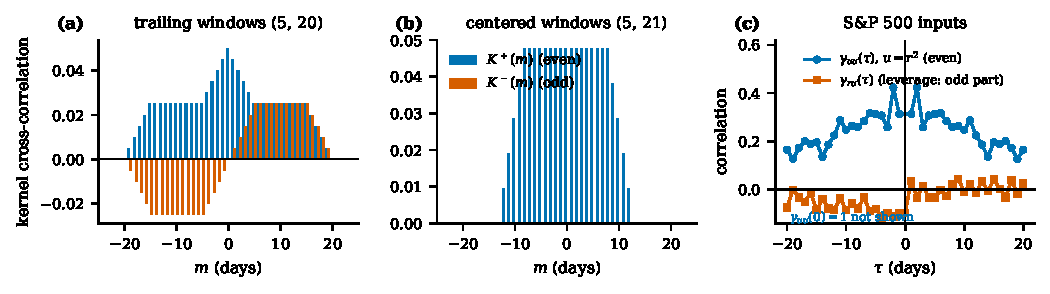
\includegraphics[width=\textwidth]{figures/fig1_decomposition.pdf}
\caption{The two ingredients of Proposition~\ref{prop:decomp}. (a) Trailing windows of 5 and 20 days: the cross-correlation $K(m)$ of the two kernels has an odd part, because the window centers differ by 7.5 days. (b) Centered windows of 5 and 21 days: $K^-\equiv0$, so no observer term arises. (c) Inputs from the S\&P 500: the autocorrelation of squared returns is even, whereas the cross-correlation $\mathrm{Corr}(r_{t+\tau},r_t^2)$ is negative for $\tau<0$ and near zero for $\tau>0$---returns precede volatility, and this odd part is the leverage effect.}
\label{fig:decomp}
\end{figure*}

\subsection{Two corollaries}\label{sec:corollaries}

Windows of one scalar signal are blind, at second order, to the irreversibility of that signal.

\begin{corollary}[Single-channel blindness]\label{cor:single}
If all observables filter the same scalar input, then $P_{ij}\equiv0$, and $C(0)$ and $C(1)$ are identical for the input and its time reversal. Every quantity computed from $C(0)$ and $C(1)$---the antisymmetry, the drift, current and entropy production of the fitted linear Markov model, and the Gaussian Markov Kullback--Leibler divergence---is therefore the same for a process and its time reversal.
\end{corollary}

\begin{corollary}[Symmetric kernels]\label{cor:symmetric}
If all kernels are symmetric about a common center (centered windows of any widths), or all kernels are equal (equal-width trailing windows), then $K_{ij}$ is even and $O_{ij}\equiv0$.
\end{corollary}

Corollary~\ref{cor:single} restates the elementary fact that the second-order statistics of a scalar stationary process are time symmetric; its content here is that every quantity a linear early-warning pipeline computes from windows of one signal inherits this symmetry, so any current such a pipeline reports is made by the observer. It is the second-order face of a general fact: a coarse-graining that does not commute with time reversal can create apparent irreversibility, whereas a commuting one bounds the true entropy production from below \cite{martinez2019,hartich2024,bisker2024,esposito2012}; Corollary~\ref{cor:symmetric} identifies the commuting linear filters. The classical observation that moving averages of random series generate spurious oscillations \cite{slutzky1937} concerns a single filtered series and is time symmetric; the effect here needs two kernels with different temporal centers. Conversely, scalar observation can hide the currents of a linear system \cite{lucente2022prr}.

\subsection{Entropy production of the fitted model}\label{sec:factor}

The entropy production of a fitted two-dimensional linear model is the squared antisymmetry times a factor set by the geometry of its innovations. Least squares of $y_{t+1}-y_t$ on $y_t$ gives, in the population, $\Phi=C(1)C(0)^{-1}$, the drift per step $A=\Phi-I$ and the residual covariance $D=C(0)-\Phi C(0)\Phi^\top$. Read as the Ornstein--Uhlenbeck (OU) process $dZ=AZ\,dt+G\,dW$ with $GG^\top=D$ and stationary covariance $\Sigma$ ($A\Sigma+\Sigma A^\top+D=0$), the fitted model carries the current $J(z)=\Omega\Sigma^{-1}z\,\rho(z)$, $\Omega=\tfrac12(A\Sigma-\Sigma A^\top)$, and the entropy production per step \cite{seifert2012}
\begin{equation}
\dot e_p=2\,\mathrm{tr}\big(\Sigma^{-1}\Omega^\top D^{-1}\Omega\big).\label{eq:ep}
\end{equation}
In two dimensions $\Omega=\omega_{\rm fit}\,\mathsf J$ with $\mathsf J=\bigl(\begin{smallmatrix}0&1\\-1&0\end{smallmatrix}\bigr)$, and $\mathsf J^\top D^{-1}\mathsf J=D/\det D$.

\begin{proposition}[Factorization]\label{prop:factor}
For a fitted two-dimensional OU model,
\begin{equation}
\dot e_p=2\,\omega_{\rm fit}^2\,\mathcal G,\qquad
\mathcal G=\frac{\mathrm{tr}(\Sigma^{-1}D)}{\det D}=\frac{1}{d_{\min}}+\frac{1}{d_{\max}},\label{eq:factor}
\end{equation}
where $d_{\min}\le d_{\max}$ are the eigenvalues of $D$ in coordinates whitened by $\Sigma$.
\end{proposition}

In standardized coordinates $\omega_{\rm fit}$ differs from the antisymmetry~\eqref{eq:omega} only through $\Sigma\neq C(0)$ (by \OmFitDevLo--\OmFitDevHi\% for the Gaussian observer below). The geometry factor $\mathcal G$ diverges when the innovations of the two observables are nearly collinear, which is exactly what happens for two windows of one signal: both are driven by the same newest input value. The size of $\dot e_p$ then reports innovation geometry rather than the strength of the current.

\subsection{Gaussian observer}\label{sec:gauss}

For a unit OU input $dx=-\lambda x\,dt+\sqrt{2\lambda}\,dW$ sampled at unit spacing [an AR(1) with $\phi=e^{-\lambda}$] and observed through trailing means of widths $(w,4w)$, every quantity is in closed form (Appendix~\ref{app:gauss}); by Corollary~\ref{cor:single}, $\omega=O$. Table~\ref{tab:gauss} lists them at $\phi=0.98$. At $\lambda w=0.1$ the antisymmetry is only \OmTabOne ($\omega_{\rm fit}=\,$\OmFitTabOne in the fitted model), yet the fitted model reports an entropy production of \EpTabOne per step for a process with none: $2\omega_{\rm fit}^2\mathcal G=\,$\EpTabOne because $\mathcal G=\,$\GTabOne. The current has the direction of the lag: an excursion of the input moves the short window first and the long one later, so the trajectory circulates counterclockwise in the $(y_1,y_2)$ plane and $\omega<0$ in every row of Table~\ref{tab:gauss}. Independent white observation noise of 1\% of the window variance changes $\omega$ by \OmNoiseOne but lowers $\dot e_p$ to \EpNoiseOne; noise of 10\% lowers $\dot e_p$ to \EpNoiseTen, while $\omega$ changes by \OmNoiseTen, only through the noise-inflated variances [Fig.~\ref{fig:gauss}(b,c)]. Centered windows give zero to sampling accuracy (Corollary~\ref{cor:symmetric}), and $3\times10^5$-step simulations reproduce the closed forms of the flux-to-drift ratio, $\dot e_p$ and the Gaussian Markov Kullback--Leibler divergence $d_1$ within \SimMaxErr (Supplemental Material \cite{SM}, Table~\Sref{gauss}). Because all observables are filters of one scalar signal, the spectral matrix of $y$ has rank one and the forward and backward path measures are mutually singular, so the full-path divergence is infinite; Eq.~\eqref{eq:factor} shows how this singularity enters the fitted model through $d_{\min}\to0$.

A metastable input behaves in the same way. For the double well of Sec.~\ref{sec:dw} with $\tau_c=\infty$, seen through two trailing windows $(w,4w)$ of $x$ alone, the input is scalar and reversible, so by Corollary~\ref{cor:single} any fitted current is made by the observer; the fitted OU model nevertheless reports $\dot e_p=\,$\DWEpOne per step at $w=1$, falling to \DWEpEighty at $w=80$ [Fig.~\ref{fig:dw}(c)]. For finite $\tau_c$ the latent $(x,c)$ process carries a genuine current, but only (\DWLatLo--\DWLatHi)$\times10^{-3}$ per step by the same estimator (Table~\Sref{dwcurrent}), three orders of magnitude less, and Proposition~\ref{prop:factor} attributes the excess to nearly collinear innovations. The Gaussian observer with the local stiffness $\bar\lambda$ predicts the short-window value (\DWPredOne at $w=1$) and falls below it at wide windows, where the slow hopping component dominates (Sec.~\ref{sec:dw}).

\begin{table*}[t]
\squeezetable
\caption{Gaussian observer, $\phi=0.98$, windows $(w,4w)$ in standardized coordinates: posterior variance $s^2$ of the latent state, lag-one antisymmetry $\omega$ [Eq.~\eqref{eq:omega}] and its fitted-model counterpart $\omega_{\rm fit}$, geometry factor $\mathcal G$ and entropy production $\dot e_p=2\omega_{\rm fit}^2\mathcal G$ (per step) of the fitted OU model, the same with observation noise $\eta^2=10^{-2}$ ($\dot e_p^{\,\eta}$), and the normalized information loss $\ell$ of a $2\sigma$ threshold forecast at a horizon of ten steps, as in Fig.~\ref{fig:gauss}(a).}
\label{tab:gauss}
\begin{ruledtabular}
\begin{tabular}{rcccccrrc}
$\lambda w$ & windows & $s^2$ & $\omega$ & $\omega_{\rm fit}$ & $\mathcal G$ & $\dot e_p$ & $\dot e_p^{\,\eta}$ & $\ell$\\
\hline
0.1 & (5,20) & 0.044 & $-$0.0135 & $-$0.0127 & $1.50\times10^{4}$ & 4.85 & 0.210 & 0.102\\
0.2 & (10,40) & 0.101 & $-$0.0121 & $-$0.0110 & $1.64\times10^{4}$ & 3.96 & 0.105 & 0.216\\
0.4 & (20,80) & 0.205 & $-$0.0098 & $-$0.0087 & $1.91\times10^{4}$ & 2.88 & 0.045 & 0.384\\
1.0 & (49,196) & 0.435 & $-$0.0058 & $-$0.0052 & $2.71\times10^{4}$ & 1.48 & 0.011 & 0.654\\
2.0 & (99,396) & 0.660 & $-$0.0031 & $-$0.0029 & $4.26\times10^{4}$ & 0.71 & 0.003 & 0.835\\
4.0 & (198,792) & 0.836 & $-$0.0015 & $-$0.0014 & $7.54\times10^{4}$ & 0.31 & 0.001 & 0.934\\
\end{tabular}
\end{ruledtabular}

\end{table*}
